\documentclass[
11pt, % Set the default font size, options include: 8pt, 9pt, 10pt, 11pt, 12pt, 14pt, 17pt, 20pt
%t, % Uncomment to vertically align all slide content to the top of the slide, rather than the default centered
%aspectratio=169, % Uncomment to set the aspect ratio to a 16:9 ratio which matches the aspect ratio of 1080p and 4K screens and projectors
]{beamer}

\graphicspath{{Images/}{./}} % Specifies where to look for included images (trailing slash required)

\usepackage{todonotes}
\usepackage{graphicx}
\usepackage{xcolor}
\usepackage{subfig}
%%\usepackage[noend]{algpseudocode}

%
%\usepackage{algorithm}
%\usepackage{algorithmic}
\usepackage{algorithm}
\usepackage{algpseudocode}
\usepackage{blkarray}
\usepackage{amsmath}
\usepackage{xspace}
\usepackage{float}


\usepackage{tikz}
\usetikzlibrary{matrix, decorations, patterns, positioning, shapes, calc, intersections, arrows, fit}

\usetikzlibrary{patterns}
\usetikzlibrary{fit,calc,positioning,decorations.pathreplacing,matrix,3d, hobby}

\usepackage{booktabs} % Allows the use of \toprule, \midrule and \bottomrule for better rules in tables
\usepackage{bm}
\usepackage{multirow}

\newcommand{\brown}[1]{{\color{brown} #1 }}

%% Colors from https://latexcolor.com/
\definecolor{pastelviolet}{rgb}{0.8, 0.6, 0.79}
\definecolor{babyblueeyes}{rgb}{0.63, 0.79, 0.95}
\definecolor{pastelyellow}{rgb}{0.99, 0.99, 0.59}
\definecolor{pastelgreen}{rgb}{0.47, 0.87, 0.47}
\definecolor{pastelred}{rgb}{1.0, 0.41, 0.38}
\colorlet{patternblue}{blue!60}


\colorlet{darkred}{red!80!black}
\colorlet{darkblue}{blue!80!black}
\newcommand<>{\darkred}[1]{{\color{darkred}{#1}}}
\newcommand<>{\darkblue}[1]{{\color#2{blue!50!black!100}{#1}}}

\newcommand{\A}{\mathbf{A}}
\newcommand{\B}{\mathbf{B}}
\newcommand{\CC}{\mathbf{C}}
\newcommand{\Real}{\mathbb{R}}
\newcommand{\vc}[1]{\bm{#1}}

\usetheme{Madrid}

\newcommand{\Tra}{{\sf T}} 


\newcommand{\Ms}[2]{\mathbf{#1}^{(#2)}} 
\newcommand{\M}[1]{\mathbf{#1}} 
\newcommand{\Mb}[2]{\mathbf{#1}_{#2}} 
\newcommand{\Mbs}[3]{\mathbf{#1}_{#2}^{(#3)}} 

%\usepackage{enumitem}



%----------------------------------------------------------------------------------------
%	PRESENTATION INFORMATION
%----------------------------------------------------------------------------------------

\title[Matrix factorization]{Matrix factorization} % The short title in the optional parameter appears at the bottom of every slide, the full title in the main parameter is only on the title page

%\subtitle{Optional Subtitle} % Presentation subtitle, remove this command if a subtitle isn't required

\author[Suraj Kumar]{Suraj Kumar} % Presenter name(s), the optional parameter can contain a shortened version to appear on the bottom of every slide, while the main parameter will appear on the title slide

\institute[Inria \& ENS Lyon]{Inria \& ENS Lyon \\ \smallskip Email:\textit{suraj.kumar@ens-lyon.fr}} % Your institution, the optional parameter can be used for the institution shorthand and will appear on the bottom of every slide after author names, while the required parameter is used on the title slide and can include your email address or additional information on separate lines

\date[CR12]{CR12: September 2024\\ \smallskip\small https://surakuma.github.io/courses/daamtc.html} % Presentation date or conference/meeting name, the optional parameter can contain a shortened version to appear on the bottom of every slide, while the required parameter value is output to the title slide

%----------------------------------------------------------------------------------------

\begin{document}
	
	%----------------------------------------------------------------------------------------
	%	TITLE SLIDE
	%----------------------------------------------------------------------------------------
	
	\begin{frame}
		\titlepage % Output the title slide, automatically created using the text entered in the PRESENTATION INFORMATION block above
	\end{frame}
	\begin{frame}{Matrix factorizations}
		\begin{itemize}
			\item Useful to solve systems of linear equations $Ax=b$
			\vfill
			\item Popular factorizations
%			\vfill
			\begin{itemize}
				\item LU factorization
				\item QR factorization
%				\item Cholesky factorization
				\item Singular value decomposition
			\end{itemize}
		\end{itemize}
	\end{frame}

	\begin{frame}{Important definitions}
		
\small
		\begin{block}{Vector norm for $x\in \mathbb{R}^n$}
%			Given a $x\in \mathbb{R}^n$, 
%			n-dimension vector $\mathbf{x}=\begin{pmatrix}
%			x_1\\
%			x_2\\
%			\vdots\\
%			x_n
%			\end{pmatrix}$,
			The Euclidean norm of $x$ is represented as $||\mathbf{x}||$ or $||\mathbf{x}||_2$ and defined as 
			$||\mathbf{x}|| = \sqrt{\sum_{i=1}^{n}x_i^2}$
		\end{block}
	\vfill
	\begin{block}{Matrix norm for $A\in \mathbb{R}^{n\times n}$}
		\begin{itemize}
			\item[] $$\textnormal{Frobenius norm, } ||A||_F = \sqrt{\sum_{j=1}^{n}\sum_{i=1}^{n}{A_{ij}}^2} = \sqrt{trace(AA^T)}$$
			\item[] $$\textnormal{Spectral norm, }||A||_2 = \textnormal{largest singular value of A}$$
		\end{itemize}
	\end{block}
\vspace*{-0.1cm}
\begin{block}{Orthogonal matrix}
			An orthogonal matrix $Q$ satisfies $Q^TQ=QQ^T=I$ (the identity matrix)
\begin{itemize}
	%		\item $Q$ must be square
	\item $Q$'s rows are orthogonal to each other and have unit norm
	\item $Q$'s columns are orthogonal to each other and have unit norm
\end{itemize}
\end{block}

	\end{frame}
\section{Singular value decomposition}

	\begin{frame}{Table of Contents}		
	\tableofcontents[currentsection,hideallsubsections] % Output the table of contents (all sections on one slide)		
\end{frame}

\begin{frame}{Singular Value Decomposition (SVD)}
	\begin{itemize}
		\item It decomposes a matrix $A$ $\in$ $\mathbb{R}^{m \times n}$ to the form $U\Sigma V^T$
		\begin{itemize}
			\item $U$ is an $m\times m$ orthogonal matrix
			\item $V$ is an $n\times n$ orthogonal matrix
			\item $\Sigma$ is an $m\times n$ rectangular diagonal matrix
		\end{itemize}
	\vfill
	\item The diagonal entries $\sigma_i=\Sigma_{ii}$ of $\Sigma$ are called singular values
	\begin{itemize}
		\item $\sigma_i\ge 0$ and $\sigma_1\ge \sigma_2\ge \cdots \ge \sigma_{\min(m,n)}$
	\end{itemize}
	\vfill
	\item Columns of $U$ and $V$ are known as left and right singular vectors respectively
	\vfill
	\item If $u_i, v_i$ are the $ith$ vector of $U$ and $V$, then $A= \sum_{i=1}^{\min(m,n)} \sigma_i u_i v_i^T$
	\vfill
	\item The largest $r$ such that $\sigma_r\ne 0$ is called the rank of the matrix
	\end{itemize}
\end{frame}
\begin{frame}{SVD and rank of a matrix}
	
	\small
	\begin{itemize}
	\item SVD represents a matrix as the sum of $r$ rank one matrices
	%		\begin{itemize}
	%			\item $A= \sum_i \Sigma(i;i)U_i V_i^T$
	%			\item Minimum number of rank one matrices required in the sum is called the rank of the original matrix
	%		\end{itemize}
\end{itemize}
\vfill
\begin{center}
	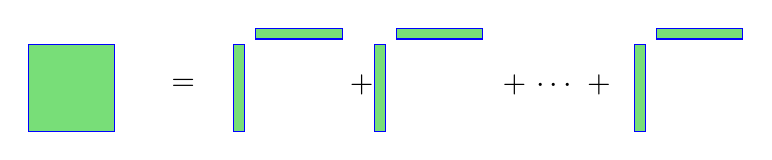
\begin{tikzpicture}[scale=0.275, every node/.style={transform shape}]
	\pgfmathsetmacro{\cubex}{4}
	\pgfmathsetmacro{\cubey}{4}
	\pgfmathsetmacro{\cubez}{4}
	\draw[blue,fill=pastelgreen] (0,0,0) -- ++(-\cubex,0,0) -- ++(0,-\cubey,0) -- ++(\cubex,0,0) -- cycle;
	%%\draw[blue,fill=pastelgreen] (0,0,0) -- ++(0,0,-\cubez) -- ++(0,-\cubey,0) -- ++(0,0,\cubez) -- cycle;
	%%\draw[blue,fill=pastelgreen] (0,0,0) -- ++(-\cubex,0,0) -- ++(0,0,-\cubez) -- ++(\cubex,0,0) -- cycle;
	
	\node[draw=none, text=black, scale=4] at (2,-3,-3) {$=$};
	\pgfmathsetmacro{\smallwidth}{0.5}
	\draw[blue,fill=pastelgreen] (\cubex+2,0,0) -- ++(-\smallwidth,0,0) -- ++(0,-\cubey,0) -- ++(\smallwidth,0,0) -- cycle;
	\draw[blue,fill=pastelgreen] (\cubex+2 +\cubex + 0.5,0.75,0) -- ++(-\cubex,0,0) -- ++(0,-\smallwidth,0) -- ++(\cubex,0,0) -- cycle;
	%%\draw[blue,fill=pastelgreen] (\cubex+2,0.5,0) -- ++(-\smallwidth,0,0) -- ++(0,0,-\cubez) -- ++(\smallwidth,0,0) -- cycle;
	
	\node[draw=none, text=black, scale=4] at (2+\cubex+4.25,-3,-3) {$+$};
	
	\draw[blue,fill=pastelgreen] (\cubex+2.5 + \cubex+2,0,0) -- ++(-\smallwidth,0,0) -- ++(0,-\cubey,0) -- ++(\smallwidth,0,0) -- cycle;
	\draw[blue,fill=pastelgreen] (\cubex+2.5+\cubex+2 +\cubex + 0.5,0.75,0) -- ++(-\cubex,0,0) -- ++(0,-\smallwidth,0) -- ++(\cubex,0,0) -- cycle;
	%%\draw[blue,fill=pastelgreen] (\cubex+2.5+\cubex+2,0.5,0) -- ++(-\smallwidth,0,0) -- ++(0,0,-\cubez) -- ++(\smallwidth,0,0) -- cycle;
	
	\node[draw=none, text=black, scale=4] at (2+\cubex+5 + \cubex+ 4.25, -3,-3) {$+$ $\cdots$ $+$};
	
	\draw[blue,fill=pastelgreen] (12 + \cubex+2.5 + \cubex+2,0,0) -- ++(-\smallwidth,0,0) -- ++(0,-\cubey,0) -- ++(\smallwidth,0,0) -- cycle;
	\draw[blue,fill=pastelgreen] (12+\cubex+2.5+\cubex+2 +\cubex + 0.5,0.75,0) -- ++(-\cubex,0,0) -- ++(0,-\smallwidth,0) -- ++(\cubex,0,0) -- cycle;
	%%\draw[blue,fill=pastelgreen] (12 + \cubex+2.5+\cubex+2,0.5,0) -- ++(-\smallwidth,0,0) -- ++(0,0,-\cubez) -- ++(\smallwidth,0,0) -- cycle;
	\end{tikzpicture}
\end{center}
\vfill
\begin{itemize}
	\item $||A||_F^2 = \sum_{i=1}^{\min(m,n)} \sigma_i^2 = \sum_{i=1}^{r} \sigma_i^2$ 
	\vfill
	\item If $r'\le r$ and $\tilde{A}= \sum_{i=1}^{r'} \sigma_i u_i v_i^T$, then $$||A-\tilde{A}||_F^2 = \sum_{i=r'+1}^{\min(m,n)} \sigma_i^2 = \sum_{i=r'+1}^{r} \sigma_i^2$$
	\vfill
	\item Useful for compression, dimension reduction and low-rank approximation
	\vfill
	\item Expensive to compute and hard to parallelize	
\end{itemize}
\end{frame}

	\section{LU factorization}
	\begin{frame}{Table of Contents}		
		\tableofcontents[currentsection,hideallsubsections] % Output the table of contents (all sections on one slide)		
	\end{frame}

\begin{frame}{Algebra of LU factorization with an example}
	Given the matrix $A = \begin{pmatrix}
	2 & 6 & 5\\
	4 & 15 & 11\\
	6 & 30 & 23
	\end{pmatrix}$
	\vfill
	\begin{itemize}
		\item Let $L_1 = \begin{pmatrix}
		1 & 0 & 0\\
		-2 & 1 & 0\\
		-3 & 0 & 1\\
		\end{pmatrix} $, $L_1A=\begin{pmatrix}
		2 & 6 & 5\\
		0 & 3 & 1\\
		0 & 12 & 8		
		\end{pmatrix}$
		\vfill
		\item Let $L_2=\begin{pmatrix}
		 1 & 0 & 0\\
		 0 & 1 & 0 \\
		 0 & -4 & 1
		\end{pmatrix}$, $L_2L_1A=\begin{pmatrix}
		2 & 6 & 5\\
		0 & 3 & 1\\
		0 & 0 & 4
		\end{pmatrix}$
		\vfill
		\item Let $U=\begin{pmatrix}
		2 & 6 & 5\\
		0 & 3 & 1\\
		0 & 0 & 4
		\end{pmatrix}$, $L_2L_1A=U$
	\end{itemize}
\end{frame}
\begin{frame}{Algebra of LU factorization}
	
	{\small
		
	$L_2L_1A=U \implies A= (L_2L_1)^{-1}U = L_1^{-1}L_2^{-1}U$
	\vfill
	 $L_1$=$\begin{pmatrix}
	1 & 0 & 0\\
	-2 & 1 & 0\\
	-3 & 0 & 1\\
	\end{pmatrix} $, $L_1^{-1}$=$\begin{pmatrix}
	1 & 0 & 0\\
	2 & 1 & 0\\
	3 & 0 & 1\\
	\end{pmatrix}$, $L_2$=$\begin{pmatrix}
	1 & 0 & 0\\
	0 & 1 & 0 \\
	0 & -4 & 1
	\end{pmatrix}$, $L_2^{-1}$=$\begin{pmatrix}
	1 & 0 & 0\\
	0 & 1 & 0 \\
	0 & 4 & 1
	\end{pmatrix}$
	\vfill 
	$\qquad\qquad\qquad\qquad\qquad\qquad L_1^{-1}L_2^{-1} = \begin{pmatrix}
	1 & 0 & 0\\
	2 & 1 & 0\\
	3 & 4 & 1\\
	\end{pmatrix}$
	\vfill 

	$A=\begin{pmatrix}
			2 & 6 & 5\\
			4 & 15 & 11\\
			6 & 30 & 23
		\end{pmatrix} = \begin{pmatrix}
		1 & 0 & 0\\
		2 & 1 & 0\\
		3 & 4 & 1\\
		\end{pmatrix}\begin{pmatrix}
		2 & 6 & 5\\
		0 & 3 & 1\\
		0 & 0 & 4
		\end{pmatrix} = LU$, where $L=L_1^{-1}L_2^{-1}$
}
\end{frame}
	\begin{frame}{The need of pivoting  (or row exchanges): $PA=LU$}
	\begin{itemize}
		\item To avoid division by $0$ or small diagonal elements (for stability)
		\item $A= \begin{pmatrix}
		0 & 2 & 4\\
		3 & 1 & 2\\
		6 & 8 & 7
		\end{pmatrix}$ has an LU factorization if we permute the rows of the matrix $A$
		$$PA=\begin{pmatrix}
		3 & 1 & 2\\
		0 & 2 & 4\\
		6 & 8 & 7
		\end{pmatrix} = \begin{pmatrix}
		1 & 0 & 0\\
		0 & 1 & 0\\
		2 & 3 & 1\\
		\end{pmatrix} 
		\begin{pmatrix}
		3 & 1 & 2\\
		0 & 2 & 4\\
		0 & 0 & -9
		\end{pmatrix}$$
		
		$\qquad\qquad\qquad$Here $P=\begin{pmatrix}
		0 & 1 & 0\\
		1 & 0 & 0\\
		0 & 0 & 1
		\end{pmatrix}$			 
	\end{itemize}
\end{frame}







	\begin{frame}{Communication lower bounds}
		\begin{itemize}
%			\item People obtain results for matrix multiplication operations
			\item Matrix multiplication lower bounds apply to LU factorization using reduction [Ballard et. al., 09]
%			, for instance, bound for LU factorization\vspace*{-0.15cm}
			{\scriptsize\begin{align*}
				\begin{pmatrix}
				I &  & -B\\
				A & I &  &\\
				& & I
				\end{pmatrix}
				&=
				\begin{pmatrix}
				I & &\\
				A & I & \\
				&& I
				\end{pmatrix}
				\begin{pmatrix}
				I & & -B \\
				& I & AB\\
				& & I
				\end{pmatrix}
				\end{align*}}
		\end{itemize}
%	\vfill
	\begin{block}{Lower bounds}
	\begin{itemize}
		\item Sequential lower bound on bandwidth = $\Omega(\frac{n^3}{\sqrt{M}})$
		\vfill
		\item Memory-dependent parallel lower bound on bandwidth = $\Omega(\frac{n^3}{P\sqrt{M}})$
		\vfill
		\item Memory-independent parallel lower bound on bandwidth = $\Omega\left(\frac{n^2}{P^\frac23}\right)$
	\end{itemize}
	\end{block}
	\end{frame}

	\begin{frame}{LU factorization}
	\begin{minipage}{0.65\linewidth}
		LU factorization (Gaussian elimination):
		\begin{itemize}
			\item Convert a matrix $A$ into product $L\times U$
			\item $L$ is lower triangular with diagonal 1
			\item $U$ is upper triangular
			\item $L$ and $U$ stored in place with $A$
		\end{itemize}
	\end{minipage}~~~
	\begin{minipage}{0.3\linewidth}
		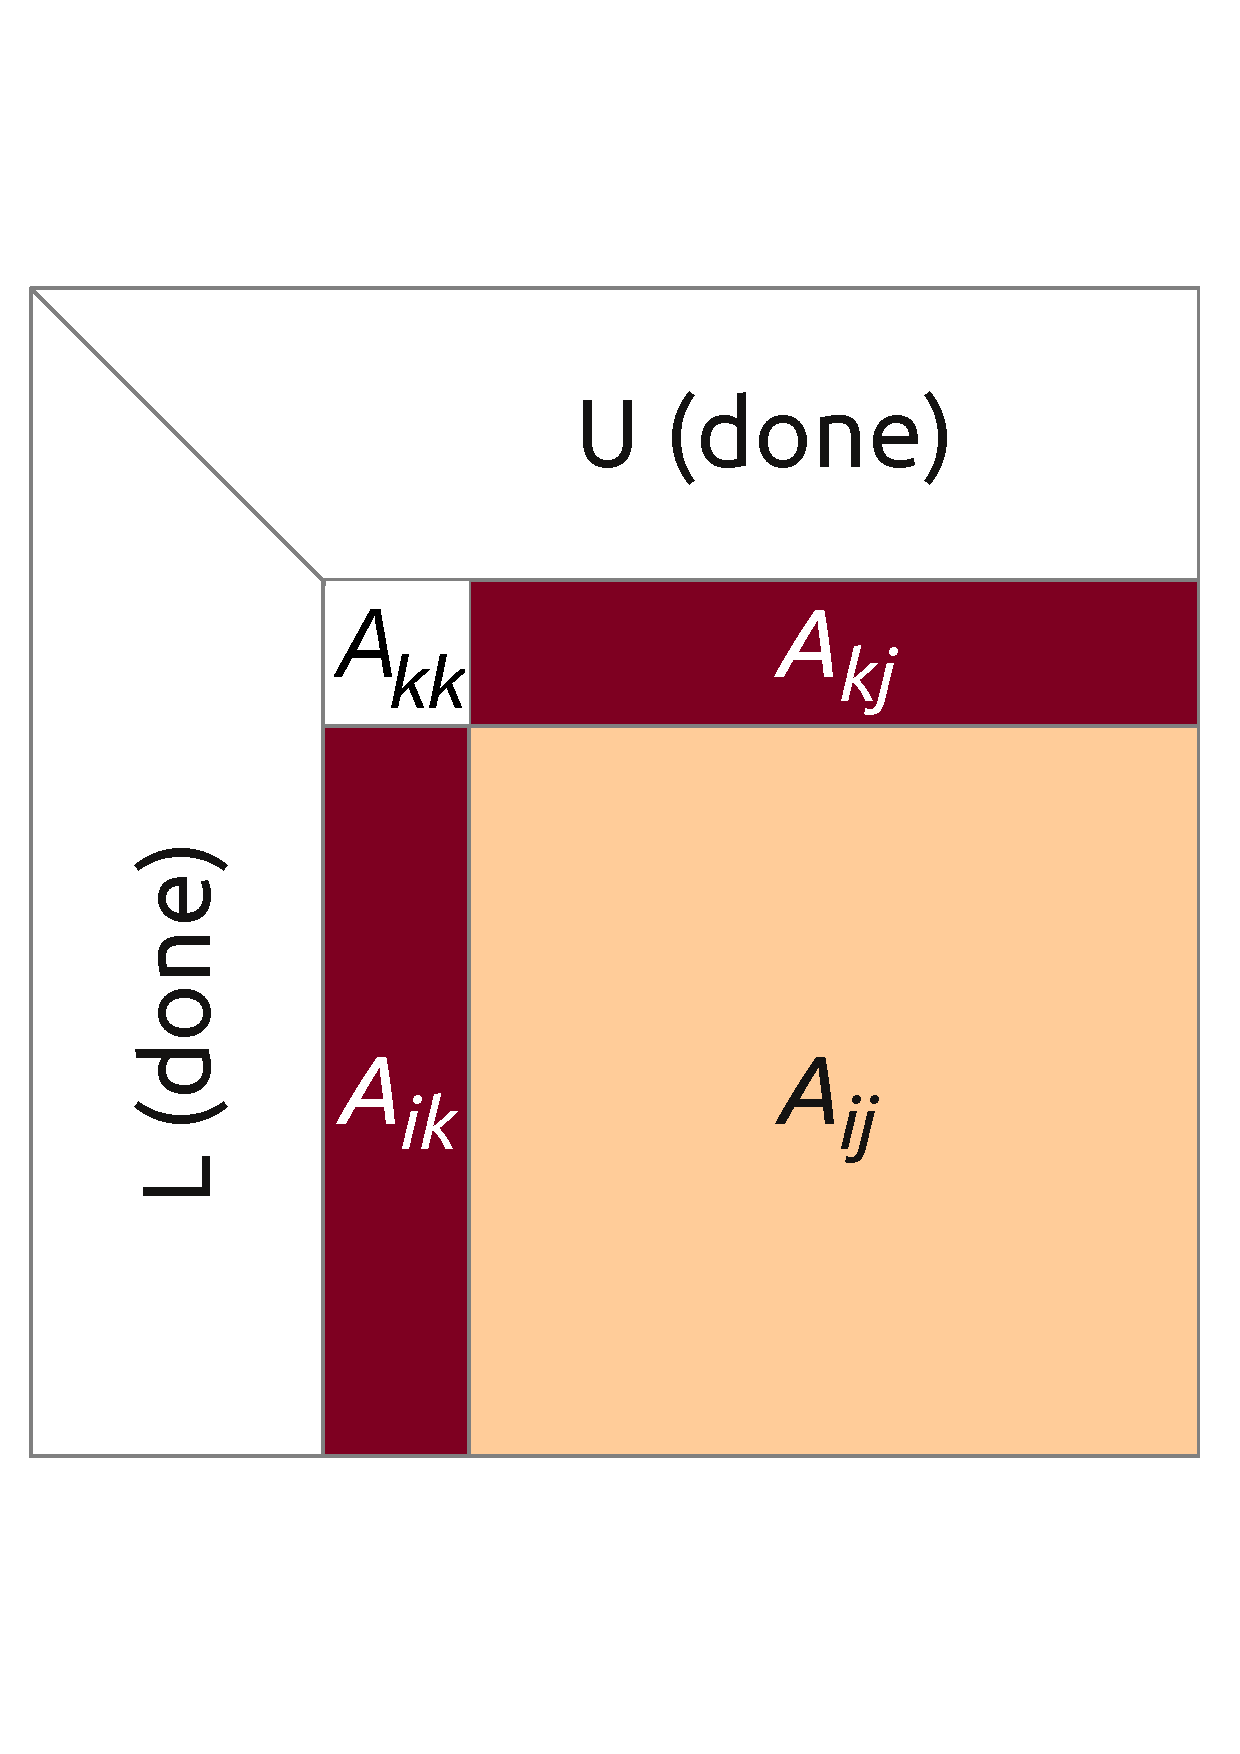
\includegraphics[width=\linewidth]{lu-final.pdf}
	\end{minipage}
	\vfill
	\begin{block}{LU Algorithm}
		For $k=1\ldots n-1$:
		\begin{itemize}
			\item For $i=k+1\ldots n$, \\
			$A_{i,k} \gets A_{i,k}/A_{k,k}$ (column/panel preparation)
			\item For $i=k+1\ldots n$, \\
			~~For $j=k+1\ldots n$, \\
			~~~~$A_{i,j} \gets A_{i,j} - A_{i,k} A_{k,j}$ (update)
		\end{itemize}
	\end{block}
\end{frame}
\begin{frame}{Block LU factorization}
	\begin{block}{Partition of a $n \times n$ matrix $A$}
		$$A=\begin{pmatrix}
		A_{11} & A_{12}\\
		A_{21} & A_{22}
		\end{pmatrix}$$
	Here $A_{11}$ is of size $b \times b$, $A_{21}$ is of size $(n-b) \times b$, $A_{12}$ is of size $b \times (n-b)$ and $A_{22}$ is of size $(n-b) \times (n-b)$. 
	\end{block}
	\vfill
	\begin{block}{Structure of LU factorization algorithm}
		\begin{itemize}
			\item The first iteration computes the factorization:
			$$A=\begin{pmatrix}
			A_{11} & A_{12}\\
			A_{21} & A_{22}
			\end{pmatrix} = \begin{pmatrix}
			L_{11} & \\
			L_{21} & I_{n-b}
			\end{pmatrix}
			\begin{pmatrix}
			U_{11} & U_{12}\\
			& A'
			\end{pmatrix}$$
			\item The algorithm continues recursively on the trailing matrix $A'$.
		\end{itemize}
	\end{block}
\end{frame}
\begin{frame}{Block LU factorization}
	\begin{enumerate}
		\item Compute the LU factorization of the first block column
		$$\begin{pmatrix}
		A_{11}\\
		A_{21}
		\end{pmatrix} = \begin{pmatrix}
		L_{11}\\
		L_{21}
		\end{pmatrix}U_{11}$$
		\vfill
		\item Solve the triangular system 
		$$L_{11}U_{12}= A_{12}$$
		\vfill
		\item Update the trailing matrix
		$$A' = A_{22}- L_{21}U_{12}$$
		\vfill
		\item Compute recursively the block LU factorization of $A'$
	\end{enumerate}
\end{frame}
	\section{QR factorization}
	
		\begin{frame}{Table of Contents}		
			\tableofcontents[currentsection,hideallsubsections] % Output the table of contents (all sections on one slide)		
		\end{frame}
	
	\begin{frame}{Terminology related to QR factorization}
		
		\small
		
		An \textbf{orthogonal} matrix $Q$ satisfies $Q^TQ=QQ^T=I$ (the identity matrix)
		\begin{itemize}
			\item $Q$ must be square
			\item $Q$'s rows are orthogonal to each other and have unit norm
			\item $Q$'s columns are orthogonal to each other and have unit norm
		\end{itemize}
		
		\vfill \pause
		
		A matrix $U$ has \textbf{orthonormal columns} if $U^TU=I$ (the identity matrix)
		\begin{itemize}
			\item $U$'s columns are orthogonal to each other and have unit norm
			\item $U$ can have more rows than columns, in which case $UU^T\neq I$
		\end{itemize}
		
		\vfill \pause
		
		Given a matrix $A$, we can \textbf{orthogonalize} its columns by finding a matrix $Q$ such that
		\begin{itemize}
			\item $Q$'s columns span the same space as $A$'s columns
			\item $Q$ has orthonormal columns
			\item there exists a matrix $Z$ such that $A=QZ$
		\end{itemize}
		
	\end{frame}
	
	
	\begin{frame}{QR factorization}
		
		The \textbf{QR factorization} is a fundamental matrix factorization:
		$$A = QR = \begin{bmatrix} \hat{Q} & \tilde{Q} \end{bmatrix} \begin{bmatrix} \hat{R} \\ 0 \end{bmatrix} = \hat{Q} \hat{R}$$
		\begin{itemize}
			\item if $A$ is $m\times n$, $m\geq n$, then $Q$ is $m\times m$, $R$ is $m\times n$, $\hat{Q}$ is $m\times n$, and $\hat{R}$ is $n\times n$
			\item $Q$ is orthogonal, $\hat{Q}$ has orthonormal columns, and $R$ is upper triangular
			\item $\hat{Q}$ is an orthogonalization of $A$
		\end{itemize}
		
	\end{frame}
	\begin{frame}
		\frametitle{Classical algorithms for QR factorization}
		
		\begin{enumerate}
			\item Gram-Schmidt process
			\begin{itemize}
				\item intuitive: each vector is orthogonalized against previous ones by subtracting out components of the vector in previous directions
				\item has numerical problems (vectors aren't always numerically orthonormal)
				\item two variants ``classical'' and ``modified'' are mathematically identical
			\end{itemize}
			\vfill
			\item Householder QR
			\begin{itemize}
				\item uses orthogonal matrices to transform input to triangular form
				\item numerically stable
			\end{itemize}
%			\vfill
%			\item Cholesky QR
%			\begin{itemize}
%				\item simplest and cheapest algorithm
%				\item has numerical problems (vectors aren't always numerically orthonormal)
%			\end{itemize}
		\end{enumerate}
		
	\end{frame}
	\begin{frame}
		\frametitle{Gram-Schmidt}
		
		\textcolor{blue}{
			\only<1>{Classical Gram-Schmidt (CGS) process}
			\only<2>{Modified Gram-Schmidt (MGS) process}
		}
		
		\begin{algorithmic}
			\Require $A = \begin{bmatrix} x_1 & x_2 & \cdots & x_n \end{bmatrix}$
			\For{$i=1$ to $n$}
			\State $v_i = x_i$
			\For{$j=1$ to $i-1$}
			\State $r_{ji} = q_j^T\textcolor{red}{\only<1>{x_i}\only<2>{v_i}}$ \Comment{compute size of projection of \textcolor{red}{\only<1>{$i$th col of $A$}\only<2>{current vector}} onto $q_j$}
			\State $v_i = v_i - r_{ji} q_j$ \Comment{remove this component from vector $v_i$}
			\EndFor
			\State $r_{ii}=\|v_i\|_2$
			\State $q_i = v_i/r_{ii}$ \Comment{normalize vector}
			\EndFor
			\Ensure $Q = \begin{bmatrix} q_1 & q_2 & \cdots & q_n \end{bmatrix}$ has orthonormal columns
			\Ensure $R$ is upper triangular and $A=QR$
		\end{algorithmic}
	\end{frame}

	\begin{frame}{Householder transformation}
		\begin{minipage}{0.57\linewidth}
			
			\begin{itemize}
				\item $v$ is a unit vector
				\vfill
				\item The reflection hyperplane can be defined by its normal vector $v$
				\vfill
				\item $(I-2vv^T)x$ is the reflection of point $x$ with the hyperplane 
			\end{itemize}
		\end{minipage}
	\begin{minipage}{0.4\linewidth}

				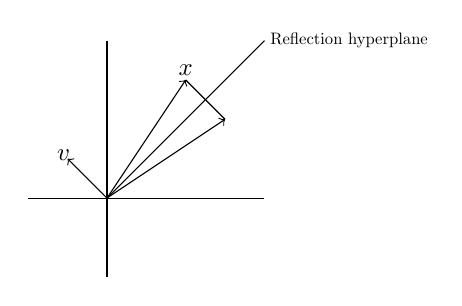
\begin{tikzpicture}[scale=0.5, every node/.style={transform shape}]
				
				\draw (0,-2) -- (0,4);
				\draw (-2,0) -- (4,0);
				\draw (0,0) -- (4,4);
				
				\draw [->] (0,0) -- (3,2);
				\draw [->] (0,0) -- (2,3);
				\draw  (3,2) -- (2,3);
				
				\draw [->] (0,0) -- (-1,1);
				
				\node [scale=1.8] at (-1.1,1.1) {$v$};
				\node [scale=1.8] at (2,3.25) {$x$};
				\node [scale=1.2,right] at (4,4) {Reflection hyperplane};
		\end{tikzpicture}
	\end{minipage}
\vfill
	\begin{itemize}
		\item $P=I-2vv^T$ matrix is known as the Householder matrix
		\vfill
		\item $P$ is symmetric and orthogonal, $P^2=I$
	\end{itemize}
	\end{frame}

\begin{frame}{Main idea of Householder QR factorization}
%	\begin{itemize}
%		\item[] 
		Look for a Householder matrix that annihilates the elements of a vector $x$, except first one:	
		$$Px=y, ||x||_2=||y||_2, y=\sigma e_1, \sigma=\pm ||x||_2$$
		
		\vfill
		
		The choice of sign is made to avoid cancellation or small numerical values while computing $v_1=x_1-\sigma$. Here $v_1$, $x_1$ are the first elements of vectors $v$, $x$ respectively. 
		
		$$v=x-y=x-\sigma e_1$$
		$$\qquad\qquad\sigma=-sign(x1)||x||_2, v=x-\sigma e_1$$
		$$\qquad u=\frac{v}{||v||_2}, P=I-2 uu^T$$
%	\end{itemize}

\end{frame}
\begin{frame}{Householder QR algorithm}
	
	Given vector $x$, a \textbf{Householder transformation} $I-2uu^T$ maps $x$ to $\sigma e_1$
	\begin{itemize}
		\item $u$ is called the \textbf{Householder vector}
%		\item a Householder transformation is an orthogonal matrix
	\end{itemize}
	
	\vfill
	
	\begin{algorithmic}
		\Require $A = \begin{bmatrix} x_1 & x_2 & \cdots & x_n \end{bmatrix}$
		\For{$i=1$ to $n$}
		\State Compute Householder vector $u_i$ from $x_i$
		\State $A = (I-2u_iu_i^T)A$ \Comment{apply Householder transformation}
%		= A - (2u_i)(u_i^TA)$ 
		\EndFor
		\State $R=A$
		\Ensure $U = \begin{bmatrix} u_1 & u_2 & \cdots & u_n \end{bmatrix}$ is lower triangular
		\Ensure $R$ is upper triangular and $R=Q^T A$ with $Q=(I-2u_1u_1^T)\cdots(I-2u_nu_n^T)$
	\end{algorithmic}
	
\end{frame}
\begin{frame}{Householder QR computational complexity}
	
	\small
	Let $A \in \mathbb{R}^{m\times n}$, we count the number of operation to update $A$ ($A = (I-2u_iu_i^T)A=A-2u_iu_i^TA$) in each iteration $i$.
	\begin{block}{Operations per iteration}
		\begin{itemize}
			\item Dot product $w= u_i^TA(i:m,i:n): 2(m-i)(n-i)$
			\item Outer product $u_iw: (m-i)(n-i)$
			\item Subtraction $A(i:m,i:n) = A(i:m,i:n) -2u_iw : (m-i)(n-i)$
		\end{itemize}
	The number of operations to multiply $2$ with $w$ is $(n-i)$, however it is a lower order term. Hence we do not consider it explicitly.
	\end{block}
	\vfill
	\begin{block}{Operations in Householder QR factorization}
		$$\sum_{i=1}^{n} = 4(m-i)(n-i) = 4 \sum_{i=1}^{n} = 4(mn - (m+n)i + i^2)$$
		$$\approx 4mn^2 - 4(m+n)\frac{n^2}{2} + 4\frac{n^3}{3} = 2mn^2 - 2\frac{n^3}{3}$$
	\end{block}
\end{frame}


\begin{frame}{QR factorization}
\begin{itemize}
	\item $Q$ can be stored in compact representation
	\vfill
	\item Structure of block QR algorithm is similar to the block LU algorithm
	\vfill
	\item Matrix communication lower bounds are also valid for the Householder/CGS/MGS QR factorization
\end{itemize}
\end{frame}
\begin{frame}{QR factorization algorithms}
	\begin{table}
		\centering
		\setlength\tabcolsep{2pt}
		\def\arraystretch{1.5}
		\begin{tabular}{|c|c|c|c|c|}
			\hline
			\textbf{Algorithm} & \textbf{\# flops} & \textbf{\# words} & \textbf{stability}  \\ \hline
			CGS & \multirow{3}{*}{$2mn^2+O(n^3)$} & $O(mn^2)$ & Bad \\ \cline{1-1} \cline{3-4}
			MGS &  & $O(mn^2)$ & Okay\\ \cline{1-1} \cline{3-4}
			%		CholQR & & $O(mn)$ & Okay \\ \cline{1-1} \cline{3-4}
			HouseholderQR & & $O(mn^2)$ & Good \\ \hline
		\end{tabular}
		%\caption{Algorithmic costs for various sequential orthogonalization routines for $m\times n$ matrix assuming $m> \sqrt M > n$.}
		\label{tab:seq-qr}
	\end{table}
	
\end{frame}
\subsection{Tall Skinny QR (TSQR) factorization}
	\begin{frame}{Table of Contents}		
	\tableofcontents[currentsection] % Output the table of contents (all sections on one slide)		
	\end{frame}
\begin{frame}{TSQR: QR factorization of a tall skinny matrix}{QR factorization of a $m\times n$ matrix with $m >>n$}

	

		The goal and process of Householder QR: 
		\begin{itemize}
			\item annihilate entries below diagonal to obtain upper triangular form
			\item work column-by-column, left-to-right
		\end{itemize}
		
		\vfill

	
	Tall-Skinny QR idea (Demmel, Grigori, Hoemmen, Langou '12):
	\begin{itemize}
		\item change the order of annihilation to minimize communication
		\item work row-by-row, top to bottom
	\end{itemize}

	\vfill
	
	
	
\end{frame}
\begin{frame}{Algebra of TSQR}
	\vspace*{-0.15cm}\begin{center}
		%!TEX root = ../../book.tex

% set relative sizes of m and n
\pgfmathsetmacro{\mdim}{16}
\pgfmathsetmacro{\ndim}{3}
% set step shift and arrow offset and label scale
\pgfmathsetmacro{\shft}{3.5}
\pgfmathsetmacro{\offset}{.33}
\pgfmathsetmacro{\lblscl}{2}

% for drawing help	
\newcommand{\drawgridhelp}{
	\coordinate (ll) at (0,-1);
	\coordinate (ur) at (5*\ndim+3*\shft,\mdim+2);
	\draw[help lines,dashed] (ll) grid (ur);
}

% draw labeled triangle
\newcommand{\drawtriangle}[2]{
	\draw (0,0) -- (\ndim,0) -- (\ndim,-\ndim) -- (0,0);
	\node[scale=\lblscl] at (3*\ndim/4,-\ndim/4) {$\Mbs{R}{#1}{#2}$};
}

% for 2 triangle reduction
\newcommand{\drawreduction}[5]{
	\drawtriangle{#1}{#2}
	\begin{scope}[shift={(0,-#5)}]
		\drawtriangle{#3}{#4}
	\end{scope}
	\draw[->] (\ndim+\offset,-\ndim/2) -- +(\shft-2*\offset,0);
	\draw[->] (\ndim+\offset,-\ndim/2-#5) -- (\ndim+\shft-\offset,-\ndim/2-3*\offset);
}

\begin{tikzpicture}[every node/.append style={transform shape},scale=.2]
	%\drawgridhelp
	
	% initial matrix
	\draw[xscale=\ndim,yscale=\mdim/4] (0,0) grid +(1,4);
	\node[scale=\lblscl] at (\ndim/2,7*\mdim/8) {$\Mb{A}{1}$};
	\node[scale=\lblscl] at (\ndim/2,5*\mdim/8) {$\Mb{A}{2}$};
	\node[scale=\lblscl] at (\ndim/2,3*\mdim/8) {$\Mb{A}{3}$};
	\node[scale=\lblscl] at (\ndim/2,\mdim/8) {$\Mb{A}{4}$};
	
	% local step
	\draw[->] (\ndim+\offset,7*\mdim/8) -- +(\shft-2*\offset,0);
	\draw[->] (\ndim+\offset,5*\mdim/8) -- +(\shft-2*\offset,0);
	\draw[->] (\ndim+\offset,3*\mdim/8) -- +(\shft-2*\offset,0);
	\draw[->] (\ndim+\offset,\mdim/8) -- +(\shft-2*\offset,0);
	
	% 1st reduction step
	\begin{scope}[shift={(\ndim+\shft,\mdim)}]
		\drawreduction{1}{2}{2}{2}{\mdim/4}
	\end{scope}
	\begin{scope}[shift={(\ndim+\shft,2*\mdim/4)}]
		\drawreduction{3}{2}{4}{2}{\mdim/4}
	\end{scope}
	
	% 2nd reduction step
	\begin{scope}[shift={(2*\ndim+2*\shft,\mdim)}]
		\drawreduction{1}{1}{3}{1}{\mdim/2}
	\end{scope}
	
	% final result
	\begin{scope}[shift={(3*\ndim+3*\shft,\mdim)}]
		\drawtriangle{1}{0}
	\end{scope}
	
	
\end{tikzpicture}
	\end{center}
{\small
$$A=\begin{pmatrix}
A_1\\
A_2\\
A_3\\
A_4
\end{pmatrix} = 
\begin{pmatrix}
\Mbs{Q}{1}{2}\Mbs{R}{1}{2}\\
\Mbs{Q}{2}{2}\Mbs{R}{2}{2}\\
\Mbs{Q}{3}{2}\Mbs{R}{3}{2}\\
\Mbs{Q}{4}{2}\Mbs{R}{4}{2}
\end{pmatrix} =
\begin{pmatrix}
\Mbs{Q}{1}{2} &&&\\
&\Mbs{Q}{2}{2}&&\\
&&\Mbs{Q}{3}{2}&\\
&&&\Mbs{Q}{4}{2}\\
\end{pmatrix}\begin{pmatrix}
\Mbs{R}{1}{2}\\
\Mbs{R}{2}{2}\\
\Mbs{R}{3}{2}\\
\Mbs{R}{4}{2}
\end{pmatrix}$$
$$\begin{pmatrix}
\Mbs{R}{1}{2}\\
\Mbs{R}{2}{2}\\
\Mbs{R}{3}{2}\\
\Mbs{R}{4}{2}
\end{pmatrix}= \begin{pmatrix}
\Mbs{Q}{1}{1}\Mbs{R}{1}{1}\\
\Mbs{Q}{2}{1}\Mbs{R}{2}{1}
\end{pmatrix} = \begin{pmatrix}
\Mbs{Q}{1}{1}&\\
&\Mbs{Q}{2}{1}
\end{pmatrix}\begin{pmatrix}
\Mbs{R}{1}{1}\\
\Mbs{R}{2}{1}
\end{pmatrix},\quad 
\begin{pmatrix}
\Mbs{R}{1}{1}\\
\Mbs{R}{2}{1}
\end{pmatrix} = \Mbs{Q}{1}{0}\Mbs{R}{1}{0} $$

$Q$ is represented implicitly as a product.
}
\end{frame}
\begin{frame}{Flexibility of TSQR}
	\small
\vspace*{-0.175cm}\begin{block}{Parallel TSQR}
	\begin{minipage}{0.475\linewidth}
		\begin{itemize}
			\item Assuming block row layout on $P$ processors
			\item Communication cost is that of binomial-tree reduction: $\beta \cdot O(n^2 \log P) + \alpha \cdot O(\log P)$
		\end{itemize}
	\end{minipage}
	\begin{minipage}{0.475\linewidth}
		\begin{center}
			%!TEX root = ../../book.tex

% set relative sizes of m and n
\pgfmathsetmacro{\mdim}{16}
\pgfmathsetmacro{\ndim}{3}
% set step shift and arrow offset and label scale
\pgfmathsetmacro{\shft}{3.5}
\pgfmathsetmacro{\offset}{.33}
\pgfmathsetmacro{\lblscl}{2}

% for drawing help	
\newcommand{\drawgridhelp}{
	\coordinate (ll) at (0,-1);
	\coordinate (ur) at (5*\ndim+3*\shft,\mdim+2);
	\draw[help lines,dashed] (ll) grid (ur);
}

% draw labeled triangle
\newcommand{\drawtriangle}[2]{
	\draw (0,0) -- (\ndim,0) -- (\ndim,-\ndim) -- (0,0);
	\node[scale=\lblscl] at (3*\ndim/4,-\ndim/4) {$\Mbs{R}{#1}{#2}$};
}

% for 2 triangle reduction
\newcommand{\drawreduction}[5]{
	\drawtriangle{#1}{#2}
	\begin{scope}[shift={(0,-#5)}]
		\drawtriangle{#3}{#4}
	\end{scope}
	\draw[->] (\ndim+\offset,-\ndim/2) -- +(\shft-2*\offset,0);
	\draw[->] (\ndim+\offset,-\ndim/2-#5) -- (\ndim+\shft-\offset,-\ndim/2-3*\offset);
}

\begin{tikzpicture}[every node/.append style={transform shape},scale=.2]
	%\drawgridhelp
	
	% initial matrix
	\draw[xscale=\ndim,yscale=\mdim/4] (0,0) grid +(1,4);
	\node[scale=\lblscl] at (\ndim/2,7*\mdim/8) {$\Mb{A}{1}$};
	\node[scale=\lblscl] at (\ndim/2,5*\mdim/8) {$\Mb{A}{2}$};
	\node[scale=\lblscl] at (\ndim/2,3*\mdim/8) {$\Mb{A}{3}$};
	\node[scale=\lblscl] at (\ndim/2,\mdim/8) {$\Mb{A}{4}$};
	
	% local step
	\draw[->] (\ndim+\offset,7*\mdim/8) -- +(\shft-2*\offset,0);
	\draw[->] (\ndim+\offset,5*\mdim/8) -- +(\shft-2*\offset,0);
	\draw[->] (\ndim+\offset,3*\mdim/8) -- +(\shft-2*\offset,0);
	\draw[->] (\ndim+\offset,\mdim/8) -- +(\shft-2*\offset,0);
	
	% 1st reduction step
	\begin{scope}[shift={(\ndim+\shft,\mdim)}]
		\drawreduction{1}{2}{2}{2}{\mdim/4}
	\end{scope}
	\begin{scope}[shift={(\ndim+\shft,2*\mdim/4)}]
		\drawreduction{3}{2}{4}{2}{\mdim/4}
	\end{scope}
	
	% 2nd reduction step
	\begin{scope}[shift={(2*\ndim+2*\shft,\mdim)}]
		\drawreduction{1}{1}{3}{1}{\mdim/2}
	\end{scope}
	
	% final result
	\begin{scope}[shift={(3*\ndim+3*\shft,\mdim)}]
		\drawtriangle{1}{0}
	\end{scope}
	
	
\end{tikzpicture}
		\end{center}
	\end{minipage}
\end{block}
\vspace*{-0.175cm}\begin{block}{Sequential TSQR}
	\begin{minipage}{0.475\linewidth}
			\begin{itemize}
			\item Assuming cache size is $\Omega(n^2)$
			\item It streams through matrix once achieving $O(mn)$ amount of data transfers 
		\end{itemize}
	\end{minipage}
	\begin{minipage}{0.475\linewidth}
	\begin{center}
		%!TEX root = ../../book.tex

% set relative sizes of m and n
\pgfmathsetmacro{\mdim}{16}
\pgfmathsetmacro{\ndim}{3}
% set step shift and arrow offset and label scale
\pgfmathsetmacro{\shft}{3.5}
\pgfmathsetmacro{\offset}{.33}
\pgfmathsetmacro{\lblscl}{2}

% for drawing help	
\newcommand{\drawgridhelp}{
	\coordinate (ll) at (0,-1);
	\coordinate (ur) at (5*\ndim+4*\shft,\mdim+2);
	\draw[help lines,dashed] (ll) grid (ur);
}	

\begin{tikzpicture}[every node/.append style={transform shape},scale=.195]
	%\drawgridhelp
	
	% initial matrix
	\draw[xscale=\ndim,yscale=\mdim/4] (0,0) grid +(1,4);
	\node[scale=\lblscl] at (\ndim/2,7*\mdim/8) {$\Mb{A}{1}$};
	\node[scale=\lblscl] at (\ndim/2,5*\mdim/8) {$\Mb{A}{2}$};
	\node[scale=\lblscl] at (\ndim/2,3*\mdim/8) {$\Mb{A}{3}$};
	\node[scale=\lblscl] at (\ndim/2,\mdim/8) {$\Mb{A}{4}$};
	
	% 1st step
	\begin{scope}[shift={(\ndim+\shft,\mdim)}]
		\draw (0,0) -- (\ndim,0) -- (\ndim,-\ndim) -- (0,0);
		\node[scale=\lblscl] at (3*\ndim/4,-\ndim/4) {$\Ms{R}{1}$};
		\draw (0,-\mdim/4) rectangle +(\ndim,-\mdim/4);
		\node[scale=\lblscl] at (\ndim/2,-3*\mdim/8) {$\Mb{A}{2}$};
	\end{scope}
	
	% 2nd step
	\begin{scope}[shift={(2*\ndim+2*\shft,\mdim)}]
		\draw (0,0) -- (\ndim,0) -- (\ndim,-\ndim) -- (0,0);
		\node[scale=\lblscl] at (3*\ndim/4,-\ndim/4) {$\Ms{R}{2}$};
		\draw (0,-2*\mdim/4) rectangle +(\ndim,-\mdim/4);
		\node[scale=\lblscl] at (\ndim/2,-5*\mdim/8) {$\Mb{A}{3}$};
	\end{scope}
	
	% 3rd step
	\begin{scope}[shift={(3*\ndim+3*\shft,\mdim)}]
		\draw (0,0) -- (\ndim,0) -- (\ndim,-\ndim) -- (0,0);
		\node[scale=\lblscl] at (3*\ndim/4,-\ndim/4) {$\Ms{R}{3}$};
		\draw (0,-3*\mdim/4) rectangle +(\ndim,-\mdim/4);
		\node[scale=\lblscl] at (\ndim/2,-7*\mdim/8) {$\Mb{A}{4}$};
	\end{scope}
	
	% 4th step
	\begin{scope}[shift={(4*\ndim+4*\shft,\mdim)}]
		\draw (0,0) -- (\ndim,0) -- (\ndim,-\ndim) -- (0,0);
		\node[scale=\lblscl] at (3*\ndim/4,-\ndim/4) {$\M{R}$};
	\end{scope}
	
	% draw arrows
	\draw[->] (\ndim+\offset,7*\mdim/8) -- +(\shft-2*\offset,0);
	\draw[->] (2*\ndim+\shft+\offset,\mdim-\ndim/2) -- +(\shft-2*\offset,0);
	\draw[->] (3*\ndim+2*\shft+\offset,\mdim-\ndim/2) -- +(\shft-2*\offset,0);
	\draw[->] (4*\ndim+3*\shft+\offset,\mdim-\ndim/2) -- +(\shft-2*\offset,0);
	\draw[->] (2*\ndim+\shft+\offset,5*\mdim/8) -- (2*\ndim+2*\shft-\offset,\mdim-\ndim/2-3*\offset);
	\draw[->] (3*\ndim+2*\shft+\offset,3*\mdim/8) -- (3*\ndim+3*\shft-\offset,\mdim-\ndim/2-3*\offset);
	\draw[->] (4*\ndim+3*\shft+\offset,\mdim/8) -- (4*\ndim+4*\shft-\offset,\mdim-\ndim/2-3*\offset);
	\draw[->,dashed] (\ndim+\offset,5*\mdim/8) -- +(\shft-2*\offset,0);
	\draw[->,dashed] (\ndim+\offset,3*\mdim/8) -- +(\ndim+2*\shft-2*\offset,0);
	\draw[->,dashed] (\ndim+\offset,\mdim/8) -- +(2*\ndim+3*\shft-2*\offset,0);
\end{tikzpicture}
	\end{center}
	\end{minipage}

\end{block}
\end{frame}



\end{document} 